%*********************************
%Format telah disesuaikan sesuai *
%Panduan penulisan               *
%Tugas Akhir Teknik Kompute ITS  *
%*********************************
 \documentclass[12pt, a4paper,twoside, bahasa]{report}
%\documentclass[12pt, a4paper,twoside]{report}

\title{Buku TA}
% Jika pakai windows untuk run
%    pertama kali dan error.
% Mohon cek miktex console jika 
%    compiler latex nya menggunakan miktex.
%------------------------------
%%%%%%%%%%%%%%%%%%%%%%%%%%%%%%%%%%%%%%%%%%%%
% FILE INI JANGAN DI UBAH
%%%%%%%%%%%%%%%%%%%%%%%%%%%%%%%%%%%%%%%%%%%%
\usepackage[indonesian]{babel}
%\usepackage[indonesian]{babel}



\usepackage[pdfauthor={Rohman Widiyanto},bookmarksnumbered,pdfborder={0 0 0}]{hyperref}
\usepackage[ruled,lined,commentsnumbered,linesnumbered]{algorithm2e}
\usepackage[utf8]{inputenc}
\usepackage{graphicx}
\usepackage{lipsum}  
\usepackage{hyphenat}
\usepackage{rotating}
\usepackage{booktabs}
\usepackage{lscape}
%\usepackage{algpseudocode}
\usepackage[ruled,lined,commentsnumbered,linesnumbered]{algorithm2e}
\usepackage{algpseudocode}
\usepackage{makeidx}
\usepackage{rotating}
\makeindex
\usepackage{epsfig}
\usepackage{subfig}
\usepackage{pdflscape}
\usepackage[doublespacing]{setspace}
\setstretch{1.5}
\usepackage{type1cm}
\usepackage{longtable}
\usepackage{lscape}
\usepackage{lettrine}
\usepackage{hyperref}
\usepackage[pageref]{backref}
\usepackage{multirow}
\usepackage[table,xcdraw]{xcolor}
\usepackage{eso-pic}
\newcommand\BackgroundIm{
	\put(0,0){
		\parbox[b][\paperheight]{\paperwidth}{%
			\vfill
			\centering
			\includegraphics[height=\paperheight,
			keepaspectratio]{./lib/background.png}%
			\vfill
}}}

\usepackage{fancyhdr} % Untuk pengaturan header dan footer yang lebih kompleks
\usepackage{etoolbox} % Untuk melakukan perubahan (patch) command internal LaTeX
\usepackage{url}
\usepackage{longtable}
\usepackage{float}
\usepackage{morefloats}
\floatstyle{boxed}
\newfloat{program}{thp}{lop}
\floatname{program}{Program}
\usepackage[fleqn]{amsmath}
\usepackage{nccmath}
\usepackage{enumitem}
\usepackage{ulem}
\usepackage[final]{pdfpages}
\usepackage{titlesec}
\usepackage{array}
\usepackage{multicol}
\usepackage{listings}
\usepackage{wrapfig}
\usepackage{array,tabularx}
\usepackage{lscape}
\usepackage{longtable}
\usepackage{caption}
\usepackage[export]{adjustbox}
\usepackage{ragged2e}
\usepackage{epsfig}
\usepackage{subfig}
\usepackage[top=35mm,left=40mm,right=30mm,bottom=30mm]{geometry}
\usepackage{pdflscape}
\usepackage[doublespacing]{setspace}
\setstretch{1.5}
\usepackage{type1cm}
\usepackage{lettrine}
\usepackage{hyperref}
\usepackage[pageref]{backref}
\usepackage{multirow}
\usepackage[table,xcdraw]{xcolor}
\usepackage{fancyhdr} % Untuk pengaturan header dan footer yang lebih kompleks
\usepackage{etoolbox} % Untuk melakukan perubahan (patch) command internal LaTeX
\usepackage{url}
\usepackage{longtable}
\usepackage{float}
\usepackage{morefloats}
\floatstyle{boxed}
\newfloat{program}{thp}{lop}
\floatname{program}{Program}
\usepackage[fleqn]{amsmath}
\usepackage{enumitem}
\usepackage{ulem}
\usepackage[final]{pdfpages}
\usepackage{titlesec}
\usepackage{array}
\usepackage{multicol}
\usepackage{listings}
\usepackage{wrapfig}
\usepackage{array,tabularx}
\usepackage{longtable}
\usepackage{caption}
%\usepackage{natbib}
%\usepackage[numbers]{natbib}
\usepackage[numbers]{natbib}

%\usepackage[sorting=none]{biblatex}

%square,sort,comma,numbers

%\renewcommand{\uline}[1]{\textit{#1}}
%\bibliographystyle{apalike}
\usepackage[export]{adjustbox}
\usepackage{ragged2e}
\usepackage[utf8]{inputenc}
\usepackage{afterpage}
\usepackage{lipsum}
%\usepackage{cite}
% More tidy url
%\usepackage{url}
%\usepackage{breakurl}
%\def\UrlBreaks{\do\/\do-\do.}

% Set paper size and margin
\usepackage{geometry}
\geometry{
	a4paper,
	left=40mm,
	top=35mm,
	right=30mm,
	bottom=30mm,
}

% untuk Cover
\newenvironment{FontCover}{\fontfamily{phv}\selectfont}{\par}
% untuk Lembar Pengesahan
\newenvironment{Kondisi}
{\par\vspace{\abovedisplayskip}\noindent
	\tabularx{\columnwidth}{>{$}l<{$} @{${}:{}$} >{\raggedright\arraybackslash}X}}
{\endtabularx\par\vspace{\belowdisplayskip}}
\newenvironment{Kondisi2}
{\par\vspace{\abovedisplayskip}\noindent
	\tabularx{\columnwidth}{>{$}l<{$} @{${}:{}$} >{\raggedright\arraybackslash}X}}
{\endtabularx\par\vspace{\belowdisplayskip}}
% Line spacing
\linespread{1.5}

% fix titlesec bug
\makeatletter
\patchcmd{\ttlh@hang}{\parindent\z@}{\parindent\z@\leavevmode}{}{}
\patchcmd{\ttlh@hang}{\noindent}{}{}{}
\makeatother

% Pengaturan format Chapter dan Section
\titleformat{\chapter}[display]{\bfseries\Large}{BAB \centering\thechapter}{0ex}{\vspace{0ex}\centering}[\vspace{3ex}]
\titlespacing*{\chapter}{0pt}{-4ex}{0pt}
\titleformat{\section}{\bfseries\normalsize}{\MakeUppercase{\thesection}}{1ex}{}
\titleformat{\subsection}{\normalsize\bfseries}
\titleformat{\subsubsection}{\normalsize\bfseries}

\titlespacing{\section}{0pt}{0pt}{1ex}
\titlespacing{\subsection}{0pt}{0pt}{1ex}
\titlespacing{\subsubsection}{0pt}{0pt}{1ex} 

% Keterangan rumus
\newenvironment{conditions}
{\par\vspace{\abovedisplayskip}\noindent
	\tabularx{\columnwidth}{>{$}l<{$} @{${}={}$} >{\raggedright\arraybackslash}X}}
{\endtabularx\par\vspace{\belowdisplayskip}}

% Caption label bold
\usepackage[labelfont=bf]{caption}
\captionsetup{labelfont=bf}

% Jarak caption dengan obyek
\captionsetup[figure]{font=small,skip=15pt}
\captionsetup[table]{font=small,skip=15pt}


\DeclareCaptionLabelSeparator{none}{}
\captionsetup{labelsep=period}
% Caption nama
\renewcommand{\figurename}{Gambar}
\renewcommand{\tablename}{Tabel}
\renewcommand{\lstlistingname}{Kode}

% Cek nomor halaman
\usepackage{changepage}

% Cek spelling
\usepackage{lipsum}
\setcounter{secnumdepth}{5}
\hyphenation{meng-gerak-kan mem-per-kenal-kan pe-ri-la-ku di-je-las-kan mem-bu-tuh-kan me-ne-rap-kan}

% Definisi untuk "halaman sengaja dikosongkan"
\def\kosong{
	\vspace*{\fill}
	\begin{center}\textit{Halaman ini sengaja dikosongkan}\end{center}
	\vfill
}

% Halaman sengaja dikosongkan
\patchcmd{\cleardoublepage}{\hbox{}}{\kosong}{}{}
% Untuk citation
%\newcommand{\tab}[1]{\hspace{.2\textwidth}\rlap{#1}}
\renewcommand*{\backreflastsep}{, }
\renewcommand*{\backreftwosep}{, }
\renewcommand*{\backref}[1]{}
%\renewcommand*{\backrefalt}[4]{
%	\ifcase #1
%	No citations.
%	\or
%	(Dikutip pada halaman #2).
%	\else
%	(Dikutip pada halaman #2).
%	\fi
%}
% Pengaturan penomoran halaman menggunakan package fancyhdr
\fancyhf{} 								% Mengosongkan header dan footer
\renewcommand{\headrulewidth}{0pt} 		% Menghapus garis horizontal pada header
\pagestyle{fancy} 						% Mengubah pagestyle dokumen menjadi fancy
\fancyfoot[CE,CO]{\thepage}				% Footer kanan pada hal. ganjil dan sebaliknya
%\patchcmd{\chapter}{plain}{fancy}{}{} 	% Mengubah pagestyle pada chapter menjadi fancy
\patchcmd{\chapter}{empty}{plain}{}{}
\usepackage{ifthen}
\newboolean{PembimbingDua}
\setboolean{PembimbingDua}{false}
\newboolean{bThesis}
\setboolean{bThesis}{true}

%\newcommand{\Tesis}
%{	\setboolean{bThesis}{true}
%}



\newboolean{PembimbingTiga}
\setboolean{PembimbingTiga}{false}

\newboolean{PengujiTiga}
\setboolean{PengujiTiga}{false}

\newboolean{PengujiEmpat}
\setboolean{PengujiEmpat}{false}

\newboolean{Nomenklatur}
\setboolean{Nomenklatur}{false}

\newboolean{bDoktor}
\setboolean{bDoktor}{false}
\newboolean{bMaster}
\setboolean{bMaster}{false}

\renewcommand{\em}[1]{\textit{#1}}
\renewcommand{\emph}[1]{\textit{#1}}

\newcommand{\Mahasiswa}[2]{
	\newcommand{\NamaMahasiswa}{#1}
	\newcommand{\NrpMahasiswa}{#2}
}
\newcommand{\PembimbingSatu}[2]
{
	\newcommand{\PbSatu}{#1}
	\newcommand{\NipPbSatu}{#2}
}
\newcommand{\PembimbingDua}[2]{
	\setboolean{PembimbingDua}{true}
	\newcommand{\PbDua}{#1}
	\newcommand{\NipPbDua}{#2}
}

\newcommand{\PembimbingTiga}[2]{
	\setboolean{PembimbingTiga}{true}
	\newcommand{\PbTiga}{#1}
	\newcommand{\NipPbTiga}{#2}
}

\newcommand{\PengujiSatu}[2]
{
	\newcommand{\PjSatu}{#1}
	\newcommand{\NipPjSatu}{#2}
}
\newcommand{\PengujiDua}[2]
{	\newcommand{\PjDua}{#1}
	\newcommand{\NipPjDua}{#2}
}
\newcommand{\PengujiTiga}[2]
{
\setboolean{PengujiTiga}{true}
\newcommand{\PjTiga}{#1}
\newcommand{\NipPjTiga}{#2}
}

\newcommand{\PengujiEmpat}[2]
{
\setboolean{PengujiEmpat}{true}
	\newcommand{\PjEmpat}{#1}
	\newcommand{\NipPjEmpat}{#2}
}
\newcommand{\KaDep}[2]
{
	\newcommand{\NmKaDep}{#1}
	\newcommand{\NipKaDep}{#2}
}
\newcommand{\CoverFooter}[1]
{\newcommand{\bdk}{#1}
}
\newcommand{\Judul}[1]
{
	\newcommand{\JdTesis}{#1}
}
\newcommand{\TanggalUjian}[1]
{
	\newcommand{\TglUjian}{#1}
}
\newcommand{\PeriodeWisuda}[1]
{
	\newcommand{\PerWisuda}{#1}
}

\newcommand{\Fakultas}[1]
{
	\newcommand{\fak}{#1}
}
\newcommand{\BeltFakultas}[1]
{
	\newcommand{\bbelt}{#1}
}
\newcommand{\Departemen}[1]
{
	\newcommand{\Dep}{#1}
}
\newcommand{\ggGelar}{xxxx}
\newcommand{\pPengesahan}{xxxxxxxx}

\newcommand{\Gelar}[1]
{
	\renewcommand{\ggGelar}{#1}
}

\newcommand{\tsss}{Disertasi disusun untuk memenuhi salah satu syarat memperoleh gelar}

\newcommand{\Disertasi}[1]
{\renewcommand{\tsss}{Disertasi disusun untuk memenuhi salah satu syarat memperoleh gelar}
	\renewcommand{\pPengesahan}{LEMBAR PENGESAHAN DISERTASI}
	\renewcommand{\ggGelar}{#1}
	 \setboolean{bMaster}{false}
	 \setboolean{bThesis}{true}
}

\newcommand{\prop}{PROPOSAL DISERTASI}
\newcommand{\ProposalDisertasi}
{	\renewcommand{\prop}{PROPOSAL DISERTASI}
	\setboolean{bMaster}{false}
	\setboolean{bThesis}{false}
}
%\newcommand{\Gelar}[1]
%{
%	 \renewcommand{\ggGelar}{#1}
%}

\newcommand{\BukuTA}
{	
	\renewcommand{\tsss}{Tugas akhir disusun untuk memenuhi salah satu syarat memperoleh gelar}
	\renewcommand{\pPengesahan}{LEMBAR PENGESAHAN TUGAS KAHIR}
    \setboolean{bMaster}{true}
    \setboolean{bThesis}{true}
    

}

\newcommand{\ProposalTA}
{	\setboolean{bMaster}{true}
	\renewcommand{\prop}{PROPOSAL TUGAS AKHIR}
	\setboolean{bThesis}{false}
}


\newboolean{JudulTesisEng}
\setboolean{JudulTesisEng}{false}

\newcommand{\JudulEng}[1]
{
	\setboolean{JudulTesisEng}{true}
	\newcommand{\JdTesisEng}{#1}
}

\newcommand{\Kode}[1]
{\newcommand{\Kodekk}{#1}
}

\newcommand{\TempatUjian}[1]
{
	\newcommand{\bTempatUjian}{#1}
}

\newcommand{\HariUjian}[1]
{
	\newcommand{\bHariUjian}{#1}
}

\newcommand{\DaftarRiwayatHidup}{
\addcontentsline{toc}{chapter}{Biodata Penulis}
\titlespacing*{\chapter}{0pt}{0ex}{5ex}
\appendix
\chapter*{BIODATA PENULIS}
%*********************************
%Gambar Foto 
	\begin{center}
		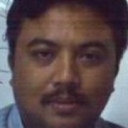
\includegraphics[height=0.2\textheight]{./ubah/Foto}
	\end{center}
%*********************************
\section*{Identitas Diri}
\begin{tabular}{p{3cm}cp{9cm}}
	%Masukan Identitas Disini.............
	Nama  		  & :&
		Eko Mulyanto Yuniarno \\
	Tempat Lahir  & :&
		Surabaya\\
	Tanggal Lahir &:& 
		12 Desember 2021\\
	Alamat        &:& J
		alan Jati No 4,Kampung Hutan, Kecamatan Danau, Kabupaten Siak\\
	Identitas 1   &:&
		 Isi Identitas 1\\
	Identitas 2   &:& 
		Isi Identitas 2\\
	Identitas 3   &:&
		 Isi Identitas 3\\
	Identitas 4   &:&
		 Isi Identitas 4\\
\end{tabular}

\section*{Riwayat Pendidikan}
\begin{tabular}{p{3cm}cp{9cm}}
	2019-Sekarang  	& :&
		Program Doktor (S3), Departemen Teknik  Elektro, Fakultas Teknologi Elektro dan Informatika Cerdas, Institut Teknologi  Sepuluh Nopember\\
	&&\\
	2014-2019  & :&
		Program Master (S2), Departemen Teknik  Elektro, Fakultas Teknologi Elektro dan Informatika Cerdas, Institut Teknologi  Sepuluh Nopember\\
	&&\\
	2011-2014  & :&
		Program Sarjana (S1), Departemen Teknik  Elektro, Fakultas Teknologi Elektro dan Informatika Cerdas, Institut Teknologi  Sepuluh Nopember\\
	&&\\
	0000-0000  & :&
		Pendidikan 1\\
	&&\\
	0000-0000  & :&
		Pendidikan 2\\
	&&\\
	0000-0000  & :&
		Pendidikan 3\\
\end{tabular}


\section*{Daftar Publikasi}

\begin{enumerate}
	\item Setiyoutami, A., Anggraeni, W., Purwitasari, D., Yuniarno, E.M., Purnomo, M.H.,\textit{Extracting Temporal-Based Spatial Features in Imbalanced Data for Predicting Dengue Virus Transmission},
	Advances in Intelligent Systems and Computing, 2021, 1158, pp. 731–742
	\item Salsabila, F.N., Yuhana, U.L., Yuniarno, E.M., Purnomo, M.H., \textit{Sifte-math, a sifteo based mathematics assessment serious game for deaf children}, IES 2020 - International Electronics Symposium: The Role of Autonomous and Intelligent Systems for Human Life and Comfort, 2020, pp. 620–625, 9231578
	
	
\end{enumerate}

\section*{Riwayat Penelitian}
\begin{enumerate}
	\item \lipsum[3]
	\item \lipsum[3]
	\item Penelitian Ke Tiga 
	\item Penelitian Ke Empat 
\end{enumerate}
\section*{Riwayat Lainnya}

\lipsum[1]
\cleardoublepage}


\newcommand{\DaftarPustaka}{%\\renewcommand\bibname{Daftar Pustaka}
%\\addcontentsline{toc}{chapter}{\bibname}
%\\titlespacing*{\chapter}{0pt}{0ex}{5ex}
%\\appendix
%\%\bibliographystyle{apalike}
%\%\bibliographystyle{ieetr}
%\%\bibliographystyle{IEEEtranN}
%\\bibliographystyle{plainnat}
%\\bibliography{./ubah/pustaka}
%\\cleardoublepage
\renewcommand\bibname{Daftar Pustaka}
\addcontentsline{toc}{chapter}{\bibname}
\titlespacing*{\chapter}{0pt}{0ex}{5ex}
\appendix
%\bibliographystyle{IEEEtranN}
\bibliographystyle{IEEEtran}
\bibliography{IEEEabrv,./ubah/pustaka}
%\bibliography{library}
\cleardoublepage}

\tolerance=9999
\emergencystretch=10pt
\hyphenpenalty=10000
\exhyphenpenalty=100


%************************************
% 1. JENIS BUKU
%    Pilih Salah Satu 
%-------------------------------------
\ProposalTA
% \BukuTA
%**********************************


%*******************************
%2.  Kode Matakuliah Tugas Akhir dan Gelar
%--------------------------------
\Kode{Tugas Akhir - EC184701}
\Gelar{Sarjana Teknik (S.T.)}
%*******************************

%*******************************
%  3. Judul Tugas Akhir Atau Proposal 
%-------------------------------
% Judul Dalam Bahasa Indonesia
\Judul{JUDUL DALAM BAHASA INDONESIA}
% Judul Dalam Bahasa Inggris
\JudulEng{JUDUL DALAM BAHASA INGGRIS}

%************************************
% 4. Identitas Mahasiswa
% Format :\Mahasiswa{Nama}{Nrp}
%------------------------------------
\Mahasiswa{Nama mahasiswa}{0000000}
%************************************
% 5. Waktu Dan Ruang Ujian
%------------------------------------
%Tanggal Ujian 
\TanggalUjian{1 Juni 2019}
% Perioda wisuda  
\PeriodeWisuda{September 2019} 
%Hari ujian dan Tempat Ujian 
\HariUjian{Senin}
\TempatUjian{Ruang B204}


%************************************
%6. Identitas Pembimbing 
%   Jumlah pembimbing Maximal = 3
%   Format : \PembimbingXXX{Nama}{Nip}
%-----------------------------------
%\scalebox{.95}[1.0]{xxx}
\PembimbingSatu{Dr. Eko Mulyanto Yuniarno Yuniarno}{196806011995121009}
\PembimbingDua{Dr. Eko Mulyanto Yuniarno}{196806011995121009}
%\PembimbingTiga{Dr. Eko Mulyanto Yuniarno,ST. MT.}{132135221}

%************************************
% 7. Identitas Penguji 
%     Huymlah penguji Maximal = 4 
%     Format : \PengujiXXX{Nama}{Nip}
%-------------------------
\PengujiSatu{Dr. Eko Mulyanto Yuniarno,ST. MT.}{196806011995121009}
\PengujiDua{Dr.Eko Mulyanto Yuniarno}{196806011995121009}
\PengujiTiga{Dr.Eko Mulyanto Yuniarno}{196806011995121009}
\PengujiEmpat{Dr.Eko Mulyanto Yuniarno}{132135221}

%************************************
% 8. Identitas Fakultas ------------------------------------
\Fakultas{Fakultas Teknologi Elektro Dan Informatika Cerdas}
\BeltFakultas{BeltFte}
%************************************
% 9. Identitas Departement
%-----------------------------------
\Departemen{Teknik Komputer}
\KaDep{ Dr. Supeno Mardi Susiki Nugroho,S.T.,M.T., Ph.D}{197003131995121001}
%***********************************
% 10. Footer Identitas Program Studi 
%  Pada Cover
%----------------------------------
\CoverFooter{\normalsize
	DEPARTEMEN TEKNIK KOMPUTER\\
	FAKULTAS TEKNOLOGI ELEKTRO DAN INFORMATIKA CERDAS\\
	INSTITUT TEKNOLOGI SEPULUH NOPEMBER\\
	SURABAYA\\
	2022}

%**********************************
%File Penting Yang Dapat di Edit:
%**********************************
%Abstrak :
%        ->\ubah\abstrak.tex
%Abstrak Bhs Inggris :
%        ->\ubah\abstrakEng.tex
%Kata Penggantar :
%        ->\ubah\pengantar.tex 
%Nomenklatur :
%        ->\ubah\Nomenklatur.tex
%Database Daftar Pustaka
%        ->\ubah\pustaka.bib
%DaftarRiwayatHidup 
%        ->\ubah\DaftarRiwayatHidup.tex
%----------------------------------
%**********************************
%Dokumen Utama
%----------------------------------
\begin{document}
%%%%%%%%%%%%%%%%%%%%%%%%%%%%%%%%%%%%%%%%%%%%
% FILE INI JANGAN DI UBAH ATAU MODIFIKASI
%%%%%%%%%%%%%%%%%%%%%%%%%%%%%%%%%%%%%%%%%%%%
\normalsize
\pagenumbering{roman}
\singlespacing
 \hyphenpenalty=1000
\tolerance=1000
\emergencystretch=2.5em
% Cover
%\addcontentsline{toc}{chapter}{Cover}
\begin{FontCover}
	\sffamily	
\thispagestyle{empty}
\begin{figure} [!t]
	
\includegraphics[keepaspectratio=true,scale=1,left]{lib/LogoITS.png}
	\caption*{}
	\label{fig:LogoITS}
\end{figure}
\vspace{1ex}
%\noindent\makebox[\linewidth]{\rule{\paperwidth}{10pt}}
\makebox[\linewidth]{\includegraphics[keepaspectratio=true,width=\paperwidth]{lib/\bbelt}}
\vspace{10ex}
\justify


\ifthenelse{\boolean{bThesis}}{\textbf{\Kodekk}}{\textbf{Proposal Tugas Akhir}}\\






\vspace{1ex}
\justify
\Large
\begin{spacing}{1}
%Masukan Judul Tesis Disini
\flushleft
\textbf{\JdTesis}
\end{spacing}
\normalsize
\vfill
\justify

%\begin{spacing}{1}
\large
\MakeUppercase{\NamaMahasiswa}\\
NRP  \uppercase{\NrpMahasiswa}
\vspace{2ex}
\justify
\normalsize

\ifthenelse{\boolean{bMaster}}{\textbf{DOSEN PEMBIMBING}}{\textbf{PROMOTOR}}\\
\PbSatu\\
\ifthenelse{\boolean{PembimbingDua}}{\ifthenelse{\boolean{bMaster}}{}{\\\textbf{Co.PROMOTOR\\}}}{}
\ifthenelse{\boolean{PembimbingDua}}{\PbDua\\}{}
\ifthenelse{\boolean{PembimbingTiga}}{\PbTiga\\}{}
 
\vfill
\justify
\bdk
\vspace{1ex}
%\rmfamily
\normalfont
\end{FontCover}
\newpage
\cleardoublepage
% Lembar pengesahan
\addcontentsline{toc}{chapter}{LEMBAR PENGESAHAN}

\ifthenelse{\boolean{bThesis}}
{ \AddToShipoutPicture*{\BackgroundIm}
\begin{center}

\Large\textbf{\pPengesahan}
%\Large\textbf{PROPOSAL TESIS}
\end{center}
\begin{center}
\tsss\\
\textbf{\ggGelar}\\
di\\
\textbf{Institut Teknologi Sepuluh Nopember}\\
\vspace{1ex}
Oleh:\\
\textbf{\NamaMahasiswa}\\ 
\textbf{NRP:\NrpMahasiswa}\\ 
\vspace{1ex}
Tanggal Ujian :\TglUjian\\
Periode Wisuda : \PerWisuda\\
\vspace{1ex}
\end{center}
\begin{center}
Disetujui oleh:\\
\textbf{Pembimbing}:
\end{center}
\begin{enumerate}
\item \PbSatu \hfill ...............................\\
NIP:\NipPbSatu \vfill
\ifthenelse{\boolean{PembimbingDua}}{\item \PbDua\hfill ...............................\\
NIP:\NipPbDua}\vfill
\ifthenelse{\boolean{PembimbingTiga}}{\item \PbTiga \hfill ...............................\\
	NIP:\NipPbTiga}{}
\end{enumerate}	
\begin{center}
	\textbf{Penguji}:
\end{center}
\begin{enumerate}
	\item \PjSatu \hfill ...............................\\
	NIP:\NipPjSatu
	\vfill
	\item \PjDua \hfill ...............................\\
	NIP:\NipPjDua\vfill
\ifthenelse{\boolean{PengujiTiga}}{
	\item \PjTiga \hfill ...............................\\NIP:\NipPjTiga\vfill}{}
\ifthenelse{\boolean{PengujiEmpat}}{
	\item \PjEmpat \hfill ...............................\\ NIP:\NipPjEmpat\vfill}{}
\end{enumerate}	
\vfill
\begin{center}
	Kepala Departemen \Dep \\
	 \fak\\
	\vspace{9ex}
	\underline{\NmKaDep}\\
	Nip:\NipKaDep
\end{center}
\newpage
}
{
\begin{center}
\textbf{LEMBAR PENGESAHAN\\
	\prop}\\    
\end{center}
\vspace{5ex}
\begin{tabular}{p{2cm} c p{8cm}}
Judul&:&\JdTesis\\
Oleh &:&\NamaMahasiswa\\
Nrp&:&\NrpMahasiswa
\end{tabular}
\vspace{5ex}
\begin{center}
\textbf{Telah Diseminarkan  Pada}
\end{center}
\begin{tabular}{p{2cm} c p{8cm}}
Hari &:&\bHariUjian\\
Tanggal &:&\TglUjian\\
Tempat&:&\bTempatUjian
\end{tabular}
\vspace{5ex}
%\scalebox{.95}[1.0]{\PjSatu}

\begin{tabular}{p{8cm} p{8cm} }
\textbf{Penguji}& \textbf{Calon Pembimbing}\\
\vspace{8ex}\hspace{-10ex}1. \PjSatu&
\vspace{8ex}\hspace{-8ex}1. \PbSatu \\
\hspace{-7ex}Nip :\NipPjSatu&
\hspace{-5ex}Nip :\NipPbSatu\\
\vspace{8ex}\hspace{-10ex}2. \PjDua&
\ifthenelse{\boolean{PembimbingDua}}
{\vspace{8ex}\hspace{-8ex}2. \PbDua}{} \\
\hspace{-7ex}Nip :\NipPjDua&
\ifthenelse{\boolean{PembimbingDua}}
{\hspace{-5ex}Nip :\NipPbDua}{}\\
\ifthenelse{\boolean{PengujiTiga}}
{\vspace{8ex}\hspace{-10ex}3. \PjTiga}{}&
\ifthenelse{\boolean{PembimbingTiga}}
{\vspace{8ex}\hspace{-8ex}3. \PbTiga}{} \\
\ifthenelse{\boolean{PengujiTiga}}
{\hspace{-7ex}Nip :\NipPjTiga}{}&
\ifthenelse{\boolean{PembimbingTiga}}
{\hspace{-5ex}Nip :\NipPbTiga}{}\\


\ifthenelse{\boolean{PengujiEmpat}}
{\vspace{8ex}\hspace{-10ex}4. \PjTiga}{}& \\
\ifthenelse{\boolean{PengujiEmpat}}
{\hspace{-7ex}Nip :\NipPjEmpat}{}&\\
\end{tabular}
\newpage
}
\cleardoublepage

\ifthenelse{\boolean{bThesis}}
{
	\ifthenelse{\boolean{bMaster}}
	{
\chapter*{PERNYATAAN KEASLIAN TUGAS AKHIR}
\addcontentsline{toc}{chapter}{PERNYATAAN KEASLIAN TUGAS AKHIR}


\begin{spacing}{1.5}
	
	Dengan ini saya menyatakan bahwa isi keseluruhan Tugas Akhir saya dengan judul \textbf{\JdTesis} adalah benar-benar hasil karya intelektual mandiri, diselesaikan tanpa menggunakan bahan-bahan yang tidak diijinkan dan bukan merupakan karya pihak lain yang saya akui sebagai karya sendiri.
	
	Semua referensi yang dikutip maupun dirujuk telah ditulis secara lengkap pada daftar pustaka. Apabila ternyata pernyataan ini tidak benar, saya bersedia menerima sanksi sesuai peraturan yang berlaku.
	
	\hspace{30ex}Surabaya \today
	
	\vspace{10ex}
	
	\hspace{35ex}\underline{\NamaMahasiswa}
	
	\hspace{35ex}Nrp :\NrpMahasiswa
	
\end{spacing}
\cleardoublepage

}
{
	
	\chapter*{PERNYATAAN KEASLIAN DISERTASI}
	\addcontentsline{toc}{chapter}{PERNYATAAN KEASLIAN DISERTASI}
	
	\begin{spacing}{1.5}
		
		Dengan ini saya menyatakan bahwa isi keseluruhan Disertasi  saya dengan judul \textbf{\JdTesis} adalah benar-benar hasil karya intelektual mandiri, diselesaikan tanpa menggunakan bahan-bahan yang tidak diijinkan dan bukan merupakan karya pihak lain yang saya akui sebagai karya sendiri.
	
	Semua referensi yang dikutip maupun dirujuk telah ditulis secara lengkap pada daftar pustaka. Apabila ternyata pernyataan ini tidak benar, saya bersedia menerima sanksi sesuai peraturan yang berlaku.
	
	\hspace{30ex}Surabaya \today
	
	\vspace{10ex}
	
	\hspace{35ex}\underline{\NamaMahasiswa}
	
	\hspace{35ex}Nrp :\NrpMahasiswa
	
\end{spacing}
\cleardoublepage
}
}{}




% Kata pengantar
\newpage

\addcontentsline{toc}{chapter}{KATA PENGANTAR}
\begin{center}
\Large\textbf{Kata Pengantar}
\end{center}
\vspace{2ex}
%Tulis kata pengantar di sini
Puji dan syukur kehadirat Allah SWT atas segala limpahan berkah, rahmat, serta hidayah-Nya, penulis  dapat menyelesaikan laporan ini dengan judul PENULISAN BUKU TESIS MENGGUNAKAN LATEX UNTUK MAHASISWA MAGISTER TEKNIK ELEKTRO FTE ITS. \vspace{1ex}
Kesempurnaan hanya milik Allah SWT, untuk itu penulis memohon segenap kritik dan saran yang  membangun. Semoga laporan ini dapat memberikan manfaat bagi kita semua.
	\vspace{26pt}
	\begin{flushright}
		\begin{tabular}[b]{c}
			Surabaya, Juni 2017
			\\
			\\
			\\
			Penulis
		\end{tabular}
	\end{flushright}

\cleardoublepage
\newpage
% Abstrak
\begin{spacing}{1}
\begin{center}
		\large\textbf{\JdTesis}
	\end{center}
	\normalsize
	\begin{adjustwidth}{-0.2cm}{}
		\ifthenelse{\boolean{bMaster}}{
		
		\begin{tabular}{lcp{0.9\linewidth}}
		Nama Mahasiswa &:& \NamaMahasiswa\\
			NRP &:&\NrpMahasiswa\\
			Pembimbing &:& 1. \PbSatu\\
			\ifthenelse{\boolean{PembimbingDua}}{& & 2. \PbDua\\}{}
			
			\ifthenelse{\boolean{PembimbingTiga}}{& & 3. \PbTiga\\}{}
			
			
			
		\end{tabular}
	}{
	\begin{tabular}{lcp{0.7\linewidth}}
		Nama Mahasiswa &:& \NamaMahasiswa\\
		NRP &:&\NrpMahasiswa\\
		Promotor &:&  \PbSatu\\
		\ifthenelse{\boolean{PembimbingTiga}}{
		\ifthenelse{\boolean{PembimbingDua}}{Co. Promotor&: & 1. \PbDua\\}{}
		\ifthenelse{\boolean{PembimbingTiga}}{& & 2. \PbTiga\\}{}
	}
{
	\ifthenelse{\boolean{PembimbingDua}}{\hspace{5ex}Co. Promotor&: & \PbDua\\}{}
	
}
	\end{tabular}

}

	
	\end{adjustwidth}
	\vspace{2ex}
	\begin{center}
		\Large\textbf{ABSTRAK}
	\end{center}
	\vspace{1ex}	
%Tulis Abstrak disini
Paragraf ke satu.Paragraf ke satu.Paragraf ke satu. Paragraf ke satu.Paragraf ke satu.Paragraf ke satu.Paragraf ke satu.Paragraf ke satu. Paragraf ke satu.Paragraf ke satu.Paragraf ke satu.Paragraf ke satu.Paragraf ke satu. Paragraf ke satu.Paragraf ke satu.

Paragraf ke dua. Paragraf ke dua. Paragraf ke dua. Paragraf ke dua.Paragraf ke dua. Paragraf ke dua. Paragraf ke dua. Paragraf ke dua.Paragraf ke dua. Paragraf ke dua. Paragraf ke dua. Paragraf ke dua.Paragraf ke dua. Paragraf ke dua. \\

%Tulis Kata Kunci disini
\vspace{2ex}
\textbf{Kata kunci }: kata kunci 1, kata kunci 2
	
\end{spacing}
\cleardoublepage
\ifthenelse{\boolean{JudulTesisEng}}
{
	\begin{spacing}{1}
\begin{center}
		\large\textbf{\JdTesisEng}
	\end{center}
	\normalsize
	\begin{adjustwidth}{-0.2cm}{}
		\begin{tabular}{lcp{0.9\linewidth}}
		By &:& \NamaMahasiswa\\
			Student Identity Number &:&\NrpMahasiswa\\
			Supervisor &:& 1. \PbSatu\\
			\ifthenelse{\boolean{PembimbingDua}}{& & 2. \PbDua\\}{}
			\ifthenelse{\boolean{PembimbingTiga}}{& & 3. \PbTiga\\}{}
		\end{tabular}
	\end{adjustwidth}
	\vspace{2ex}
	
	\begin{center}
		\Large\textbf{ABSTRACT}
	\end{center}
	\vspace{1ex}	
%Tulis Abstrak disini
Paragraf ke satu.Paragraf ke satu.Paragraf ke satu. Paragraf ke satu.Paragraf ke satu.Paragraf ke satu.Paragraf ke satu.Paragraf ke satu. Paragraf ke satu.Paragraf ke satu.Paragraf ke satu.Paragraf ke satu.Paragraf ke satu. Paragraf ke satu.Paragraf ke satu.

Paragraf ke dua. Paragraf ke dua. Paragraf ke dua. Paragraf ke dua.Paragraf ke dua. Paragraf ke dua. Paragraf ke dua. Paragraf ke dua.Paragraf ke dua. Paragraf ke dua. Paragraf ke dua. Paragraf ke dua.Paragraf ke dua. Paragraf ke dua. \\

%Tulis Kata Kunci disini
\vspace{2ex}
\textbf{Keyword}: Keyword 1, Keyword 2
\end{spacing}
}{}
\cleardoublepage

% Daftar isi
\renewcommand*\contentsname{DAFTAR ISI}
\titlespacing*{\chapter}{0pt}{0ex}{0ex}
\tableofcontents
\cleardoublepage
% Daftar gambar
\renewcommand*\listfigurename{DAFTAR GAMBAR}
\addcontentsline{toc}{chapter}{\listfigurename}
\titlespacing*{\chapter}{0pt}{0ex}{0ex}
\listoffigures
\cleardoublepage
% Daftar tabel
\renewcommand*\listtablename{DAFTAR TABEL}
\addcontentsline{toc}{chapter}{\listtablename}
\titlespacing*{\chapter}{0pt}{0ex}{0ex}
\listoftables
\cleardoublepage
% Nomenklatur
\addcontentsline{toc}{chapter}{NOMENKLATUR} % kata pengantar
\begin{center}
\Large\textbf{NOMENKLATUR}
\end{center}
\vspace{1ex}
\begin{conditions}
		M &	Markov \textit{Decision Process}.\\
		S &	\textit{State}.\\
		\alpha& Learning Rate
\end{conditions}
\newpage

\cleardoublepage

% Bab isi buku
\titleformat{\chapter}[display]{\bfseries\Large}{BAB \centering\thechapter}{0ex}{\vspace{0ex}\centering}[\vspace{0ex}]
\titleformat{\section}{\bfseries\large}{\MakeUppercase{\thesection}}{1ex}{}
\titleformat{\subsection}{\bfseries\large}{\MakeUppercase{\thesubsection}}{1ex}{}
\titleformat{\subsubsection}{\bfseries\large}{\MakeUppercase{\thesubsubsection}}{1ex}{}
\titlespacing*{\chapter}{0pt}{-4ex}{0pt}
\titlespacing{\section}{0pt}{0pt}{0pt}
\titlespacing{\subsection}{0pt}{0pt}{0pt}
\titlespacing{\subsubsection}{0pt}{0pt}{0pt}
% Indent paragraph
\setlength{\parindent}{0.8cm}
\begin{spacing}{1.5}
	
\begin{spacing}{1.2}
  \chapter{PENDAHULUAN}
\end{spacing}


\pagenumbering{arabic}
\vspace{4ex}

\section{Latar Belakang}
LaTeX adalah sistem penyusunan huruf yang berkualitas tinggi; itu termasuk fitur yang dirancang untuk produksi dokumentasi teknis dan ilmiah. LaTeX adalah standar de facto untuk komunikasi dan publikasi dokumen ilmiah. LaTeX tersedia sebagai perangkat lunak gratis.

\section{Rumusan Masalah}
Bagian ini untuk menulis rumusan masalah.
\section{Tujuan}
Tujuan dari tutorial ini adalah \cite{Koza1996}
\begin{enumerate}
	\item Tujuan Pertama
	\item Tujuan Kedua
\end{enumerate}
\section{Batasan Masalah}
Tutorial ini dibatasi pada penggunaan Latex untuk penulisan tesis. 
\section{Manfaat}
Diharapkan mahasiswa dapat mudah menulis tesis sehingga dapat cepat menyelesaikan studi di Magister Teknik Elektro ITS.
\subsection{Contoh Subseksi }
\subsubsection{Contoh SubSub Seksi}

\begin{equation}
y=cos(\alpha x)
\end{equation}

	\cleardoublepage
	\chapter{KAJIAN PUSTAKA}


\section*{ }
Demi mendukung tutorial ini, dibutuhkan beberapa teori penunjang sebagai bahan acuan dan referensi. Dengan demikian tutorial ini menjadi lebih terarah. 
\vspace{1ex}

\section{Cara Menulis Daftar}
\underline{Menulis Dartar Item}
\begin{itemize}
	\item Ini Urutan Pertama. Ini Urutan Pertama. Ini Urutan Pertama. Ini Urutan Pertama. Ini Urutan Pertama. Ini Urutan Pertama. Ini Urutan Pertama. 
	\item Menulis Item kedua.Menulis Item kedua.Menulis Item kedua.Menulis Item kedua.Menulis Item kedua.Menulis Item kedua.Menulis Item kedua.
	\item Ini Urutan Ketiga
\end{itemize}

\underline{Menulis daftar urutan}
\begin{enumerate}
	\item Ini Urutan Pertama
	\item Ini Urutan kedua
	\begin{enumerate}
		\item Sub Urutan Pertama
		\item Sub Urutan Kedua
	\end{enumerate} 
	\item Ini Urutan Ketiga
\end{enumerate}


\section{Cara Penulisan Persamaan}
Cara menulis persamaan  inline pada text $\sum_{i=1}^{N} x_iy_i$


Contoh Integral
\begin{equation}\label{eq:persamaan1}
y=\int_{0}^{2\pi} cos(x) dx
\end{equation}
Persamaan \ref{eq:persamaan1} adalah contoh menulis fungsi $cos(\alpha x)$ dari $0\le x\le 2\pi$.\\
Menjajarkan persamaan
\begin{align}
y&=\int_{0}^{2\pi}cos(x)dx\\
&=sin(x)|_0^{2\pi}\\
&=sin(2\pi)-sin(0)\\
&=0
\end{align}
Persamaan \ref{eq:matrix} adalah matrix.
\begin{equation}\label{eq:matrix}
\textbf{X}=\begin{bmatrix}
x_{11}&x_{12}&\cdots&x_{1m}\\
x_{21}&x_{22}&\cdots&x_{2m}\\
\vdots&\vdots&\ddots&\vdots\\
x_{n1}&x_{n2}&\cdots&x_{nm}
\end{bmatrix}
\end{equation}
\vspace{1ex}
\section{Cara Penulisan Tabel}
\begin{table}[H]
	\caption{Tabel Contoh}
	\begin{tabular}{|l|l|l|l|}
		\hline
		No & X & Y & C \\ \hline
		1 & 0 & 0 & 1 \\ \hline
		2 & 0 & 1 & 0 \\ \hline
		3 & 1 & 0 & 0 \\ \hline
		4 & 1 & 1 & 0 \\ \hline
	\end{tabular}
\end{table}


\begin{table}[H]
	\label{tab:tabelcontoh2}
	\caption{Tabel ini contoh 2}
	\begin{tabular}{|l|l|l|l|}
		\hline
		\multirow{2}{*}{\textbf{No}} & \multicolumn{3}{l|}{\textbf{Data}} \\ \cline{2-4} 
		& \textbf{x} & \textbf{y} & \textbf{z} \\ \hline
		\textbf{1} & \textbf{0.1} & \textbf{0.2} & \textbf{0.3} \\ \hline
		\textbf{2} & \textbf{0.4} & \textbf{0.5} & \textbf{0.6} \\ \hline
	\end{tabular}
\end{table}
Pada Tabel \ref{tab:tabelcontoh2} di tunjukan cara membuat tabel.


\begin{sidewaystable}
	\centering
	\caption{Tabel ke samping}
	\begin{tabular}{|l|l|l|l|}
		\hline
		\multirow{2}{*}{\textbf{No}} & \multicolumn{3}{l|}{\textbf{Data}} \\ \cline{2-4} 
		& \textbf{x} & \textbf{y} & \textbf{z} \\ \hline
		\textbf{1} & \textbf{0.1} & \textbf{0.2} & \textbf{0.3} \\ \hline
		\textbf{2} & \textbf{0.4} & \textbf{0.5} & \textbf{0.6} \\ \hline
	\end{tabular}
	
\end{sidewaystable}
\newpage
\section{Cara Meletakan Gambar}
\begin{figure}[H]
	\centering
	
\includegraphics[width=0.5\linewidth]{bab2/LambangTeknikElektro}
	\caption{Lambang Teknik dengan Ukuran 0.5 Lebar Kertas}
	\label{fig:lambangteknikelektro}
\end{figure}
\begin{figure}[H]
	\centering
	
\includegraphics[width=0.2\linewidth]{bab2/LambangTeknikElektro}
	\caption{Lambang Teknik dengan Ukuran 0.2 lebar kertas}
	\label{fig:lambangteknikelektro2}
\end{figure}
\begin{figure}[H]
	\centering
	
\includegraphics[width=0.5\linewidth]{bab2/LambangTeknikKOmputer}
	\caption{Lambang Teknik Komputer  }
	\label{fig:lambangteknikkomputer}
\end{figure}
\section{Cara Membuat  sitasi}

Ini adalah cara  sitasi ke buku menggunakan cite\{Refferensi\}\\

Contoh : sitasi ke 1
 \cite{Brathwaite2009}.\\
Daftar referensi terletak pada file 
\textit{lainnya/pustaka.bib}\\

contoh  sitasi ke 2
\cite{Friedman1997}
\newline
\section{Algoritma}
Contoh Algoritma

\begin{algorithm}[H]
	\SetKwInOut{Input}{Input}
	\SetKwInOut{Output}{Output}
	
	\underline{function Euclid} $(a,b)$\;
	\Input{Two nonnegative integers $a$ and $b$}
	\Output{$\gcd(a,b)$}
	\eIf{$b=0$}
	{
		return $a$\;
	}
	{
		return Euclid$(b,a\mod b)$\;
	}
	\caption{Euclid's algorithm for finding the greatest common divisor of two nonnegative integers}
\end{algorithm}
\newpage
\section{Tools Online Yang Cukup Membantu}
Beberapa tools yang dapat digunakan untuk menulis tesis dengan latex.
\subsection{Online equation editor: HostMath }
\begin{center}
	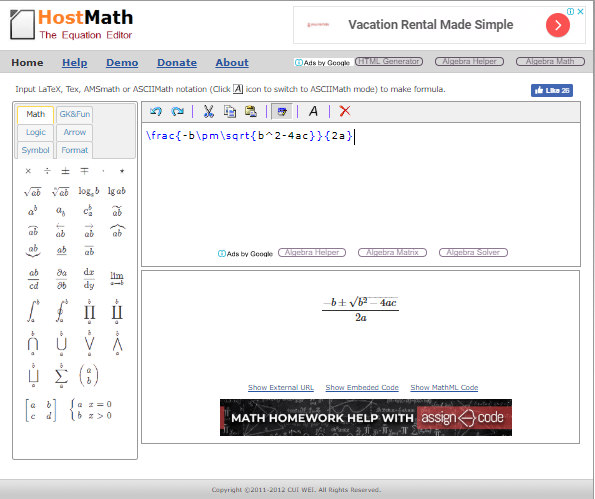
\includegraphics[width=1\linewidth]{bab2/Hosmath}
	\captionof{figure}{http://hostmath.com/}
	\label{fig:hosmath}
\end{center}




\newpage
\subsection{Detexify LaTeX handwritten symbol recognition}
\begin{center}
	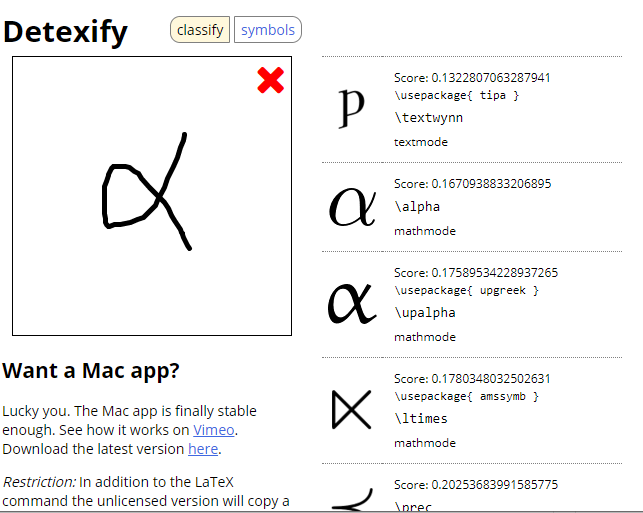
\includegraphics[width=\linewidth]{bab2/Detexify}
	\captionof{figure}{http://detexify.kirelabs.org/classify.html}
	\label{fig:detexify}
\end{center}
\newpage
\subsection{Tables Generator }
\begin{center}
	
	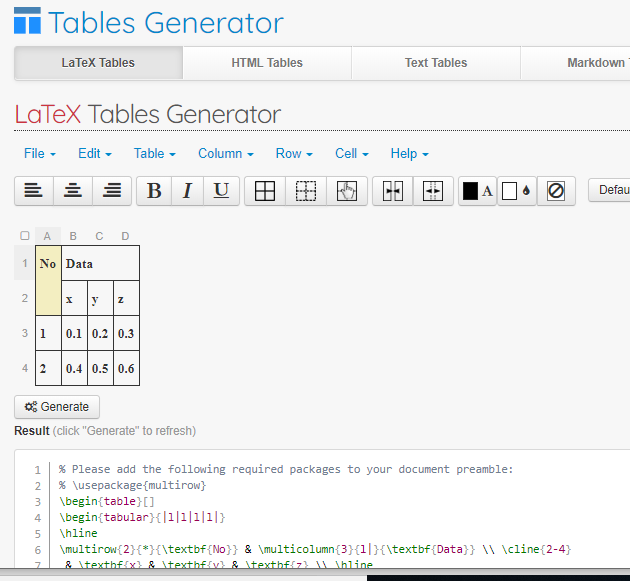
\includegraphics[width=0.7\linewidth]{bab2/TabelGenerator}
	\captionof{figure}{https://www.tablesgenerator.com/}
	\label{fig:tabelgenerator}
\end{center}

\subsection{Long Table}
\begin{landscape}

\begin{spacing}{1}	
\begin{longtable}{|p{3cm}| p{7cm} | p{7cm} | p{7cm}|}\label{table:Posisidankontribusipenelitian}\\
	\caption{Posisi dan kontribusi penelitian}\\
	%\toprule
	\hline
	\nohyphens{\textbf{Topik riset Registrasi}}  & \textbf{Metode}  &\nohyphens{\textbf{Kontribusi Peneliti Lain}}&\nohyphens{\textbf{Kontribusi Peneliti}} \\ 
	%\midrule
	\hline
	\endfirsthead
	\caption{Posisi dan kontribusi penelitian \textit{(Lanjutan..)}}\\
	%\toprule
	\hline
	
	\nohyphens{\textbf{Topik riset Registrasi}}  & \textbf{Metode}  &\nohyphens{\textbf{Kontribusi Peneliti Lain}}&\nohyphens{\textbf{Kontribusi Peneliti}} \\ 
	%\midrule
	\hline
	\endhead
	\multicolumn{4}{r}{{(\textit{Tabel bersambung..})}} \\
	\endfoot
	\endlastfoot 
	Ekstraksi feature& 	Kurvature  pada suatu titik di hitung pada beberapa skala dengan fitting  permukaan ke  titik lokal pada berbagai macam ukuran. (Ho dan Gibbins, 2009) & 	Multi-scale  Feature Extraction from 3D Meshes and Unstructured Point Cloud& \\ \hline 
	Estimasi vektor normal& 	Fitting tangen vektor pada  data titik untuk menentukan vektor normal berbasis local voronoy mesh. (OuYang dan Feng, 2005) & 	Metoda baru untuk estimasi vektor normal. & \\ \hline 
	Estimasi principal direction& 	The Adjacent-Normal Cubic Approximation 
	(Goldfeather dan Interrante, 2004) & 	Estimasi principal direction dan vektor normal pada permukaan dengan noise yang tinggi.&\\ \hline 
	Registrasi berbasis fitur permukaan. & 	Normal distribution transform.
	(Pathak, Birk,Vaskevicius dan Poppinga, 2010) & 	Online registrasi pose untuk menentukan posisi robot. & 	 \\ \hline 
	Registrasi 3D berbasis warna. & 	Warna rgb (Johnson dan Kang, 1997). 
	(Douadi dkk., 2006) & 	Menggantikan fitur geometri ketika informasi geometri permukaan tidak mencukupi. & 	\\ \hline 
	& 	Registrasi berbasis warnoHSV. (Druon, Aldon dan Crosinier, 2006) & 	Registrasi tidak di pengaruhi oleh intensitas warna. & 	\\ \hline 
	& 	Registrasi dengan Modified color ICP kombinasi antara warna RGB dengan jarak ecludiean.  (Joun,Ang,Kang,Chung dan Yu(2009) & 	Registrasi untuk lingkungan 3D. & 	\\ \hline 
	Registrasi Berbasis geometri permukaan.& 	Registrasi dengan angular invariant feature.  (Jiang dkk., 2009) & 	\textit{Angular  invariant feature} invariant terhadap rotasi dan skala. & 	\\ \hline 
	& 	Point  Feature Histograms (PFH)  robust multi-dimensional features. (Rusu, Blodow, Marton, Soos dan Beetz, 2007) & 	Kombinasi curvature, vektor normal dan vektor pcincipal direction. & 	\\ \hline 
	& 	Fitting quadratik surface  (Chen dan Bhanu, 2007) & 	Permukaan lokal sebagai deskriptor untuk Kombinasi curvature, vektor normal dan vektor pcincipal direction. & 	\\ \hline 
	& 	& 	& 	Registrasi Citra  2D multiview untuk penangkap gerak manusia
	Semina Sesindo 2010 (Yuniarno, Mardi, Sumpeno dan Hariadi, 2010)\\ \hline 
	& 	& 	& 	Registrasi permukaan berbeasis surface curvature feature.
	Jurnal Jatit  (Yuniarno, Hariadi dan Purnomo, 2013a) \\ \hline 
	Outlier Removal& 	Tiga konstrain untuk memperoleh korspondensi akurat. 
	(Liu, 2008)& 	Korespondensi yang akurat& 	\\ \hline 
	& 	Dua  konstrain untuk memperoleh korspondensi akurat. 
	(Xin dan Pu, 2010)& 	Perbaikan tiga konstrain yang diusulkan oleh Liu dengan meletakan origin ke titik berat permukaan.& 	\\ \hline 
	& 	& 	& 	perbaikan korespondensi 
	dengan rigid constraint berbasis dua titik referensi dan surface curvature feature Jurnal Kursor (Yuniarno, Hariadi dan Purnomo, 2013b)\cite{Brathwaite2009} \\ \hline 
\end{longtable}

\end{spacing}

\end{landscape}
\section{Tabel Rencana Penelitian }


\begin{table}[h!]
	\caption{Rencana Penelitian}
	\begin{tabular}{|l|l|l|l|l|l|l|l|l|l|}
		\hline
		& \multicolumn{9}{c|}{\textbf{Semester Ke}} \\ \cline{2-10} 
		\multirow{-2}{*}{} & 1 & 2 & 3 & 4 & 5 & 6 & 7 & 8 & 9 \\ \hline
		Rencana 1 & \cellcolor[HTML]{000000} & \cellcolor[HTML]{000000} & \cellcolor[HTML]{000000} & \cellcolor[HTML]{000000} & \cellcolor[HTML]{000000} &  &  &  &  \\ \hline
		Rencana 2 &  &  & \cellcolor[HTML]{000000} & \cellcolor[HTML]{000000} & \cellcolor[HTML]{000000} & \cellcolor[HTML]{000000} & \cellcolor[HTML]{000000} &  &  \\ \hline
		Rencana 3 &  &  &  &  &  & \cellcolor[HTML]{000000} & \cellcolor[HTML]{000000} & \cellcolor[HTML]{000000} & \cellcolor[HTML]{000000} \\ \hline
		Rencana 4 &  & \cellcolor[HTML]{000000} & \cellcolor[HTML]{000000}{\color[HTML]{000000} } & \cellcolor[HTML]{000000}{\color[HTML]{000000} } & \cellcolor[HTML]{000000}{\color[HTML]{000000} } & \cellcolor[HTML]{000000}{\color[HTML]{000000} } & \cellcolor[HTML]{000000}{\color[HTML]{000000} } & \cellcolor[HTML]{000000}{\color[HTML]{000000} } & \cellcolor[HTML]{000000}{\color[HTML]{000000} } \\ \hline
	\end{tabular}
\end{table}




	\cleardoublepage
	\chapter{METODOLOGI}
\label{sec:chap3_metodologi}

\section*{ }
Pada penelitian ini nantinya akan terdiri dari lima langkah utama yaitu :
\begin{figure}[H]
	\centering
	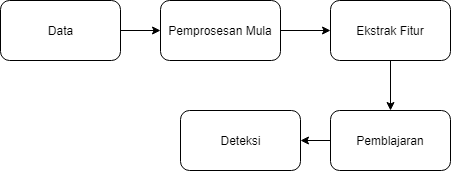
\includegraphics[width=\linewidth]{bab3/BlokDiagram}
	\caption{Blok Diagram Penelitian}
	\label{fig:blokdiagram}
\end{figure}


\section{Data}
Data adalah citra yang diperoleh dari kamera dengan ukuran $300\times 300$ dari beberapa sudut pandang yang berlainan.
\section{Pemprosesan Mula}
Citra yang telah diperoleh telah terpapar oleh gaussia noise sehingga perlu diperbaiki.
\section{Ekstraksi Fitur}
\lipsum[2]
\subsection{Fitur Warna}
\lipsum[1]
\subsection{Fitur Permukaan}
\section{Pembelajaran}
\lipsum[4]
\section{Deteksi}
\lipsum[2]







	\cleardoublepage
	\chapter{PENGUJIAN}
\label{sec:chap4_pengujian}
\vspace{1ex}

\section*{}
Berbagai metodologi yang diterapkan.
\section{Pengujian Terhadap Gausian Noise}
\lipsum[1]
\section{Pengujian Terhadap dst...}
\subsection{dst1..}
\lipsum[2]
\subsection{dst2}
\lipsum[3]


	\cleardoublepage
	\chapter{PENUTUP}
\label{sec:chap5_tutup}
\vspace{1ex}
\section*{}
Setelah penerapan metode terhadap masalah yang ingin diselesaikan pada \vspace{1ex}

\section{Kesimpulan}
\label{sec:sec4_kesimpulan}
\vspace{1ex}
\lipsum[1]
\section{Saran}
\label{sec:sec4_saran}
\vspace{1ex}
\lipsum[2]


	\cleardoublepage
	%Bab Lain bisa ditambah disini
\end{spacing}
\DaftarPustaka
%Daftar Riwayat Hidup
%    ->\ubah\DaftarRiwayatHidup.tex
\DaftarRiwayatHidup
\end{document}